\documentclass{beamer}
\setbeamercovered{transparent}
\usepackage{epstopdf}
\usepackage{listings}
\usepackage{lipsum}
\usepackage{subfig}
\usepackage{algorithm}
\usepackage{algorithmicx}
\usepackage{cite}
\usepackage{lipsum}
\usepackage{amssymb}
\usepackage{color}
\usepackage{IEEEtrantools}
\usepackage{booktabs}
\usepackage{texpower}
\usepackage{amsmath}
\usepackage{caption}
\usepackage{multirow}
\usepackage{graphicx}
\newtheorem{Key points}{Key points}
\newtheorem{Summary}{Summary}
\usepackage{dblfloatfix}
%\usepackage{adjustbox}
%\usepackage{animate}
%\usepackage{movie15}
%\usepackage{subfig}
%\newtheorem{Definition}{Definition}
%\usepackage[font={small}]{caption}
\usepackage{beamerthemeshadow}
\newcommand\Fontvi{\fontsize{5}{6.2}\selectfont}
\newcommand\Fontvia{\fontsize{6}{7.2}\selectfont}
\newcommand\Fontviaa{\fontsize{8}{7.2}\selectfont}
\usepackage{listings}
\lstset{language=C++,
                keywordstyle=\color{blue},
                stringstyle=\color{red},
                commentstyle=\color{magenta},
                morecomment=[l][\color{magenta}]{\#},
                numbers=left,
                escapeinside=||
}

%\captionsetup{font=scriptsize,labelfont=scriptsize}
 \usetheme{Antibes}%PaloAlto
\begin{document}
\title[Lecture 2]{Data Structures} 
\author[]{Ahsan Ijaz}
\date{}
 \frame{\titlepage}
% \AtBeginSection[]
% {
% \begin{frame}<beamer>{Table of Contents}
% \tableofcontents[currentsection,currentsubsection, 
%     hideothersubsections, 
%     sectionstyle=show/shaded,
% ]
% \end{frame}
% }

 \section{Sequential Containers}
 \frame{\frametitle{Sequential Containers} A container holds a
   collection of objects of a specified type. The
   \textbf{{\color{blue}sequential containers}} let the programmer
   control the order in which the elements are stored and
   accessed. That order does not depend on the values of the
   elements. Instead, the order corresponds to the position at which
   elements are put into the container.
   \begin{itemize}
   \item Each container has different trade-offs relative to:
     \begin{itemize}
     \item The costs to add or delete elements to the container
     \item The costs to perform nonsequential access to elements of
       the container
     \end{itemize}
   \end{itemize}
 } \frame{\frametitle{Types of Sequential Containers}
   \begin{figure}
     \centering
     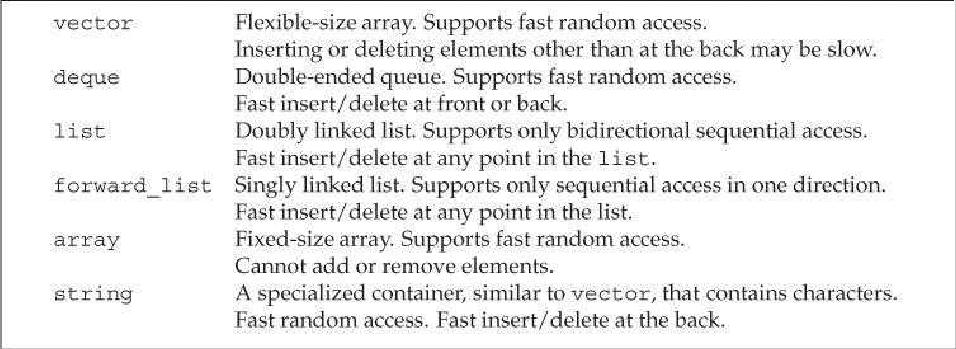
\includegraphics[width=1\columnwidth]{d.jpg}
     \caption{Types of Sequential Containers}
     \label{fig:d}
   \end{figure}
 } \frame{\frametitle{Sequential Containers} Containers provide:
   \begin{itemize}
   \item Efficient, flexible memory management.
   \item We can add and remove elements
   \item Size of containers can grow and shrink.
   \end{itemize}
 } \frame{\frametitle{Strings and Vectors} String and vector hold
   their elements in contiguous memory.\\ \textbf{Pros:}
   \begin{itemize}
   \item Since elements are contiguous, it is fast to compute the
     address of an element from its index.
   \end{itemize}

   \textbf{Cons:}
   \begin{itemize}
   \item Adding or removing elements in the middle of one of these
     containers takes time:
     \begin{enumerate}
     \item All the elements after the one inserted or removed have to
       be moved to maintain contiguity.
     \item adding an element can sometimes require that additional
       storage be allocated. In that case, every element must be moved
       into the new storage.
     \end{enumerate}
   \end{itemize}
  }
\frame{\frametitle{list and forward\_List} \textbf{Pro:} The list
   and forward\_list containers are designed to make it fast to add or
   remove an element anywhere in the container.\\  \textbf{Con:}
   \begin{itemize}
   \item In exchange, these types do not support random access to
     elements: We can access an element only by iterating through the
     container.
   \item The memory overhead for these containers is often
     substantial, when compared to vector, deque, and array.
   \end{itemize}
 } \frame{\frametitle{Rule of thumb for selection of Container}
   \begin{itemize}
   \item<1-> Unless you have a reason to use another container, use a
     vector.
   \item<2-> If your program has lots of small elements and space overhead
     matters, don’t use list or forward\_list.
   \item<3-> If the program requires random access to elements, use a
     vector or a deque.
   \item<4-> If the program needs to insert or delete elements in the
     middle of the container, use a list or forward\_list.
   \item<5-> If the program needs to insert or delete elements at the
     front and the back, but not in the middle, use a deque.
   \end{itemize}
 }
\subsection{Container Operations}
\begin{frame}
  \frametitle{Container Operations}
Each container provides a set of common operations (methods) for using the data stored in them. 
\end{frame}
 \begin{frame}
\frametitle{Construction of Containers}
   \begin{figure}
     \centering
     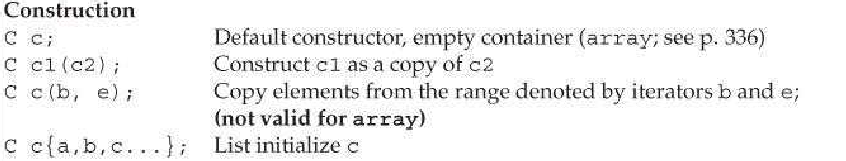
\includegraphics[width=1\columnwidth]{construction}
     \caption{Construction}
   \end{figure}
 \end{frame}

 \begin{frame}
\frametitle{Assignment and swap operations}
   \begin{figure}
     \centering
     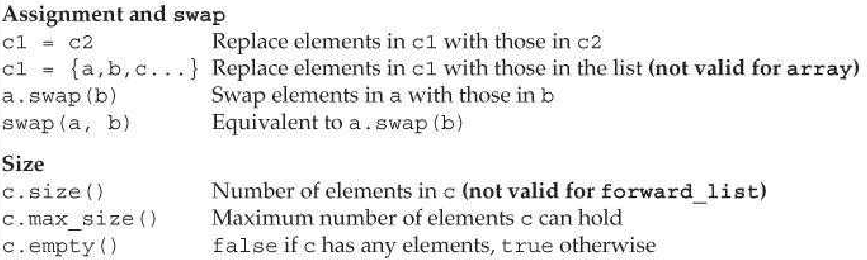
\includegraphics[width=1\columnwidth]{cons2}
     \caption{Assignment and Swap Operations}
   \end{figure}
 \end{frame}

 \begin{frame}
\frametitle{Addition and removal of elements}
   \begin{figure}
     \centering
     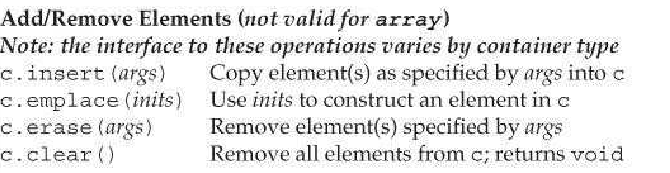
\includegraphics[width=1\columnwidth]{add}
     \caption{Adding and removing elements}
   \end{figure}
 \end{frame}

  \begin{frame}[fragile]
  \frametitle{Defining Containers}
 \begin{lstlisting}
  list<Sales_data> // list that holds Sales_data
  deque<double> // deque that holds doubles
 \end{lstlisting}
\begin{lstlisting}
  vector<vector<string>> lines; // vector of vectors
 \end{lstlisting}
   Here lines is a vector containing vectors of strings.
\end{frame}

\subsection{Iterators}
 \begin{frame}[fragile]
\frametitle{Iterators:motivation}
\begin{itemize}
\item Need a way to navigate through the items in a container.
An example: navigating over vector v.
\begin{lstlisting}
for (int i = 0; i != v.size(); i++ )
	cout << v[i] << endl;
\end{lstlisting}
\item However, doubly-linked list would need a different form to fetch data.
We want a general approach to navigate elements for different implementations of a container.
\end{itemize}
\end{frame} 
 \begin{frame}[fragile]
\frametitle{Iterators}
    \begin{definition}
      Like Pointers, iterators gives indirect access to objects in a
      container.
    \end{definition}
   We can use an iterator to fetch an element and iterators have
   operations to move from one element to another.
\begin{lstlisting} 
vector<int>::iterator it; // it can read and write vector<int> elements
vector<int>::const_iterator it2; // it2 can read
// but not write elements
\end{lstlisting}
\end{frame}
 \begin{frame}[fragile]
\frametitle{Iterators job}
 A generalized type that helps in navigating a container
\begin{itemize}
\item A way to initialize at the front and back of a list
\item A way to move to the next or previous position
\item A way to detect the end of an iteration
\item A way to retrieve the current value
\end{itemize}
\end{frame}
 \begin{frame}[fragile,fragile,fragile]
\frametitle{Getting an iterator}
{\color{red}Two methods in all STL containers.}
\begin{itemize}
\item iterator begin ( )
Returns an iterator to the first item in the container
\item iterator end ( )
Returns an iterator representing end marker in the container (that is, the position after the last item)
\end{itemize}
\begin{lstlisting}
for (int i = 0; i != v.size(); i++ )
	cout << v[i] << endl;
\end{lstlisting}
can be written as:
\Fontviaa
\begin{lstlisting}
for(vector<int>::iterator itr=v.begin(); itr!=v.end(); itr++)
{
cout << *itr++ << endl;
}
\end{lstlisting}
\end{frame}
 \begin{frame}[fragile,fragile]
\frametitle{auto keyword}
\textbf{{\color{blue}auto}} keyword automatically checks and assigns the appropriate type to the variable.
\begin{lstlisting}
// type is explicitly specified
list<string>::iterator it5 = a.begin();
list<string>::const_iterator it6 = a.begin();
// iterator or const_iterator depending on a's type of a

auto it7 = a.begin(); // const_iterator only if a is const
auto it8 = a.cbegin(); // it8 is const_iterator
\end{lstlisting} 
When we use auto with begin or end, the iterator type we get depends on the
container type.
\end{frame}
\subsection{Initializing Containers}
\begin{frame}[fragile]
  \frametitle{Initialize container}
\begin{lstlisting}
// ten int elements, each initialized to -1
vector<int> ivec(10, -1); 
 // ten strings; each element is "hi!"
list<string> svec(10, "hi!");
// ten elements, each initialized to 0
forward_list<int> ivec(10); 
// ten elements, each an empty string
deque<string> svec(10); 

\end{lstlisting}
\end{frame}

\begin{frame}[fragile,fragile]
  \frametitle{Initializing a container from another container}
\Fontviaa
\begin{lstlisting}
  /* each container has three elements, initialized 
from the given initializers*/
list<string> authors = {"Milton", "Shakespeare", "Austen"};
vector<const char*> articles = {"a", "an", "the"};
list<string> list2(authors); // ok: types match
deque<string> authList(authors); //error: container types mismatch
vector<string> words(articles); // ok: converts const char*
// elements to string

\end{lstlisting}
\end{frame}
\subsection{Relational Operators}
\begin{frame}
  \frametitle{Relational Operators}
  \begin{itemize}
  \item  The right- and left-hand operands must be the same kind of container
and must hold elements of the same type. That is, we can compare a vector$<$int$>$ only with another vector$<$int$>$. We cannot compare a vector$<$int$>$ with a
list$<$int$>$ or a vector$<$double$>$.
  \end{itemize}
Comparing two containers performs a pairwise comparison of the elements. 
\begin{itemize}
\item  If both containers are the same size and all the elements are equal, then the
two containers are equal; otherwise, they are unequal.
\item  If the containers have different sizes but every element of the smaller one is
equal to the corresponding element of the larger one, then the smaller one is
less than the other.
\end{itemize}
\end{frame} 
\begin{frame}[fragile]
  \frametitle{Relational Operators-Example}
\begin{lstlisting}
vector<int> v1 = { 1, 3, 5, 7, 9, 12 };
vector<int> v2 = { 1, 3, 9 };
vector<int> v3 = { 1, 3, 5, 7 };
vector<int> v4 = { 1, 3, 5, 7, 9, 12 };
v1 < v2 
/* true; v1 and v2 differ at 
element [2]: v1[2] is less than v2[2] */
v1 < v3 
/* false; all elements are equal, but 
v3 has fewer of them; */
v1 == v4 
/* true; each element is equal and v1 and v4
 have the same size() */
v1 == v2 // false; v2 has fewer elements than v1
\end{lstlisting}
\end{frame}

\begin{frame}[fragile]
  \frametitle{Element type Dependency}
  \begin{itemize}
  \item We can use a relational operator to compare two containers only if the
appropriate comparison operator is defined for the element type.
  \end{itemize}

\begin{lstlisting}
vector<Sales_data> storeA, storeB;
if (storeA < storeB) // error: Sales_data has
                    // no less-than operator

\end{lstlisting}
\end{frame}
\end{document}